%instiki:category: FisicaSubatomica
% use latex2itexv2 chapter1.tex to obtain inkstiki file
% use latex2itexTOC to obtain Tabla de Contenidos
\chapter{Teor\'\i a Cl\'asica de Campos}
\label{chap:tcc} %noinstiki
%instiki:
%instiki:***
%instiki:
%instiki:[[NotasFS|Tabla de Contenidos]]
%instiki:
%instiki:***
%instiki:
%generated with html2itexTOC instiki_source.html
%instiki:* [Principio de M\'\i nima Acci\'on](#la)
%instiki:
%instiki:* [La cuerda cl\'asica unidimensional](#la-cuerda-clasica)
%instiki:
%instiki:* [Principio de M\'\i nima Acci\'on para ...](#principio-de-minima-call)
%instiki:
%instiki:* [Aplicaci\'on a Mec\'anica Cu\'antica](#aplic-mecan-cuant)
%instiki:
%instiki:* [Aplicaci\'on a la cuerda unidimenisonal](#aplicacion-la-cuerda)
%instiki:
%instiki:***
%instiki:
\section{Principio de M\'\i nima Acci\'on}
\label{sec:la}

El Principio de M\'\i nima acci\'on establece, una vez fijado el espacio de
coordenadas generalizadas sobre el espacio de configuraci\'on, que de
todas las trayectorias posibles que transcurren entre $t_1$ y $t_2$,
el sistema escoger\'a aquella que minimice la acci\'on $S$
\cite{ActionPhysics}.  La magnitud de la acci\'on viene dada para cada
trayectoria por la integral:
\begin{equation}
  \label{eq:la}
   S\left[q_i,\dot{q}_i\right] = \int_{t_{1}}^{t_{2}} L(q_i(t), \dot{q}_i(t),t) dt
\end{equation}
Donde:
$q_i(t)$ son las coordenadas param\'etricas de una trayectoria posible.
$L(q_i,\dot{q}_i,t)$, es la funci\'on lagrangiana del sistema.


Puede probarse mediante principios variacionales, que de todas las trayectorias posibles, la que hace  estacionaria la anterior expresi\'on es la que satisface la siguiente condici\'on $i$:
\begin{equation}
  \label{eq:eel}
 \frac{d}{dt} \left ( \frac{\partial L}{\partial\dot{q}_i} \right ) - \frac{\partial L}{\partial q_i} = 0
\end{equation}
conocidas como las ecuaciones de Euler-Lagrange. La demostraci\'on se
har\'a m\'as adelante para el caso en el que las coordenadas generalizadas
corresponden a funciones de campo. 

De momento mostraremos como la segunda ley de Newton~\cite{NewtonSeconLaw}, puede escribirse en la forma de la ec.~(\ref{eq:eel}).
\begin{align}
\label{eq:fma}
  F&=ma\\
  -\frac{\partial V(x)}{\partial x}&=m\frac{d^2x}{dt^2}\nonumber\\
  &=m\frac{d\dot{x}}{dt}\nonumber\\
  &=\frac{d}{dt}
  \left[
    \frac{\partial}{\partial\dot{x}}
    \left(
      \frac{1}{2}m\dot{x}^2
    \right)
  \right]\nonumber
\end{align}
Podemos introducir el Lagrangiano a cada lado de la igualdad adicionando t\'erminos con la respectiva derivada parcial cero:
\begin{equation*}
  \frac{\partial}{\partial x}
  \left(
\frac{1}{2}m\dot{x}^2-V(x)
  \right)=\frac{d}{dt}
  \left[
    \frac{\partial}{\partial\dot{x}}
    \left(
      \frac{1}{2}m\dot{x}^2-V(x)
    \right)
  \right].
\end{equation*}
Reemplazando $L=\frac{1}{2}m\dot{x}^2-V(x)=T-V$, obtenemos
\begin{equation*}
\frac{d}{dt}\frac{\partial L}{\partial\dot{x}}  -\frac{\partial L}{\partial x}=0.
\end{equation*}
Una forma m\'as rigurosa de escribir la ec.~\eqref{eq:fma} puede encontrarse en~\cite{ActionPhysics}. 

El Hamiltoniano del sistema se obtiene definiendo la variable can\'onica conjugada de $x$
\begin{align}
  p=\frac{\partial\mathcal{L}}{\partial\dot{x}}=m \dot{x},
\end{align}
y usando la transformada de Legendre
\begin{align}
  H=p \dot{x}-L=\frac{\partial\mathcal{L}}{\partial\dot{x}}\dot{x}-L=\frac{1}{2}m\dot{x}^2+V=T+V
\end{align}

Para visualizar el principio de m\'\i nimo de acci\'on se recomienda seguir las actividades del programa interactivo en \texttt{Java} disponible online en \cite{JavaAP}. All\'\i{} se considera el problema de un objeto de 0.2Kg lanzado hacia arriba y retornado al punto de partida 3 segundos despues. Si dividimos la trayectoria en tres intervalos como se muestra en la Fig.~\ref{fig:apple1}, teniendo en cuenta que la velocidad es la pendiente del segmento, para $\Delta t=0.75\,$s $x_1=11.13\,$m, $t_1=0.75\,$s, $x_2=0\,$m, $t_2=1.5\,$s, tenemos que para la trayectoria mostrada
\begin{align}
  S=\int_{t_1}^{t_2}(T-V)dt\approx&\sum_i(T-V)_i\Delta t\nonumber\\
  \approx&\sum_{i=1}^2\left[\frac{1}{2}m\left(\frac{x_i-x_{i-1}}{t_i-t_{i-1}}\right)^2-m g x_i\right]\Delta t\nonumber\\
  \approx&16.67\,\text{J\,s}
\end{align}
\begin{figure}
  \centering
  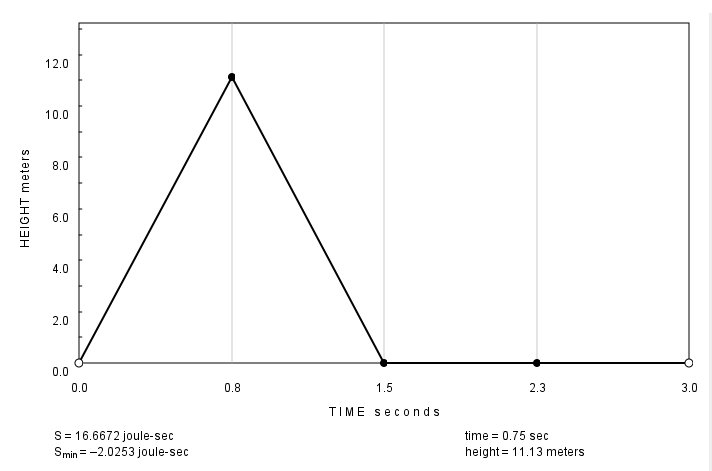
\includegraphics[scale=0.5]{apple1}
  \caption{Ejemplo de c\'alculo de la Acci\'on para una trayectoria arbitraria}
  \label{fig:apple1}
\end{figure}
Iterando el proceso se puede encontrar num\'ericamente (o a mano) la trayectoria que minimiza la acci\'on mostrada en la Fig.~\ref{fig:apple2}
\begin{figure}
  \centering
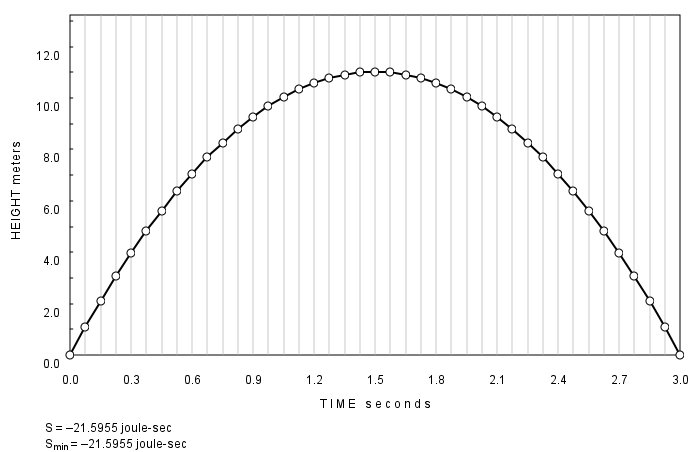
\includegraphics[scale=0.5]{apple2}
  \caption{Trayectoria que minimiza la Acci\'on}
\label{fig:apple2}
\end{figure}
Para una dimensi\'on podemos definir la densidad Lagrangiana como
\begin{equation}
  \mathcal{L}(q,\dot q,t)=\frac{\partial}{\partial q}L(q,\dot q,t)\qquad\text{or}\qquad L(q,\dot q,t)=\int\mathcal{L}(q,\dot q,t)dq.
\end{equation}
La ec.~\eqref{eq:la} puede escribirse entonces como
\begin{equation}
   S\left[q_i,\dot{q}_i\right] = \int \mathcal{L}(q_i(t), \dot{q}_i(t),t)\, dq\,dt.
\end{equation}
Para sistemas continuos es conveniente usar la densidad Lagrangiana. Abordaremos a continuaci\'on el sistema continuo correspondiente a la cuerda cl\'asica unidimensional para construir la densidad Lagrangiana correspondiente. A partir de ella demostraremos las ecuaciones de Euler Lagrange para dicho sistema.

%\left(\right)

\section{La cuerda cl\'asica unidimensional}
\label{sec:la-cuerda-clasica}

Considere una cuerda de longitud $L$ formando un c\'\i rculo de radio $R$.
Es conveniente considerar un conjunto de $N$ part\'\i culas de masa $m$ a
lo largo de la circunferencia, unidas por resortes de longitud $l$ y
constante el\'astica $k$. Los modos vibracionales de la cuerda a lo
largo de la circunferencia se obtienen en l\'\i mite de $N\to\infty$ y $l\to0$ 
%noinstiki

\begin{figure} %noinstiki
  \centering %noinstiki
  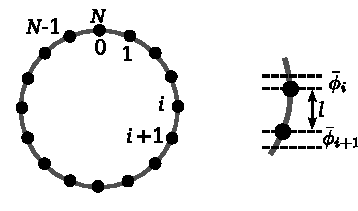
\includegraphics{cuerda} %noinstiki
  \caption{Modelo Cuerda} %noinstiki
  \label{fig:1string} %noinstiki
\end{figure} %noinstiki<div id="fig:1string">Figura cuerda: Modelo cuerda</div>
%noinstiki![cuerda](http://gfif.udea.edu.co/figfs/cuerda.png)
%noinstiki
De acuerdo a la figura 
\ref{fig:1string}, %noinstiki([cuerda](#fig:1string)),
si $\bar{\phi_i}=\bar{\phi}(z_i,t)$ es el
desplazamiento de la $i$--esima masa desde su posici\'on de equilibrio,
entonces el Lagrangiano del sistema de $N$ particulas y resortes es:
\begin{align}
  \label{eq:1strLsum} %noinstiki
  L&=\frac{1}{2}m\sum_{i=0}^{N-1}
  \left(
\frac{\partial\bar\phi_i}{\partial t}
  \right)^2-\frac{1}{2}k\sum_{i=0}^{N-1}
  \left(
\bar\phi_{i+1}-\bar\phi_{i}
  \right)^2,\\
  \label{eq:1strLsumdot} 
&=\frac{1}{2}m\sum_{i=0}^{N-1}
  \left(
    \dot{\bar{\phi_i}}
  \right)^2-\frac{1}{2}k\sum_{i=0}^{N-1}
  \left(
\bar\phi_{i+1}-\bar\phi_{i}
  \right)^2.
\end{align}
Si $\mu$ es la densidad de la cuerda, $T$ la tensi\'on y $v$ la velocidad, entonces
\begin{align}
  \label{eq:micromacro}
  \mu&=\frac{m}{l}\nonumber\\
  T&=kl\\
  v^2&=\frac{T}{\mu}.\nonumber
\end{align}
(\ref{eq:micromacro})
En el l\'\i mite $l\to0$ y $N\to\infty$, tenemos
\begin{equation}
  \label{eq:barf}
  \bar\phi_i=\bar\phi(z_i,t)\to\bar\phi(z,t),
\end{equation}
que representa la funci\'on de campo del desplazamiento de una masa
infinitesimal de su posici\'on de equilibrio. Entonces
\begin{align}
L&=\frac{1}{2}\sum_{i=0}^{N-1}\frac{m}{l}l
  \left(
    \dot{\bar{\phi_i}}
  \right)^2-\frac{1}{2}\sum_{i=0}^{N-1}(k l) l
  \left(
\frac{\bar\phi_{i+1}-\bar\phi_{i}}{l}
  \right)^2.\nonumber\\
&=\frac{1}{2}\sum_{i=0}^{N-1}\mu
  \left(
    \dot{\bar{\phi_i}}
  \right)^2l-\frac{1}{2}\sum_{i=0}^{N-1}T
  \left(
\frac{\bar\phi_{i+1}-\bar\phi_{i}}{l}
  \right)^2l.
\label{eq:1strLsumm}
\end{align}
En el l\'\i mite continuo $\sum(\cdots)\,l\to\int(\cdots)\,dz$, entonces 
\begin{equation}
\label{eq:238}
  L=\int_0^L\frac{1}{2}
\left[
  \mu\left(\frac{\partial\bar\phi}{\partial t}\right)^2- T\left(\frac{\partial\bar\phi}{\partial z}\right)^2
\right]dz=\int_0^L\mathcal{L}dz,
\end{equation}
con
\begin{equation}
  \label{eq:call1}
  \mathcal{L}=\frac{1}{2}
\left[
  \mu\left(\frac{\partial\bar\phi}{\partial t}\right)^2- T\left(\frac{\partial\bar\phi}{\partial z}\right)^2
\right],
\end{equation}
y
\begin{equation}
  \label{eq:Scall}
  S=\int\mathcal{L}\,dtdz.
\end{equation}
Definiendo
\begin{equation}
  \label{eq:barff}
  \phi=\sqrt{T}\bar\phi,
\end{equation}
tenemos
\begin{align}
  \label{eq:call2}
  \mathcal{L}(\partial\phi/\partial t,\partial\phi/\partial z)=&
\frac{1}{2}
\left[
  \frac{\mu}{T}\left(\frac{\partial\phi}{\partial t}\right)^2- \frac{T}{T}\left(\frac{\partial\phi}{\partial z}\right)^2
\right]\nonumber\\
=&\frac{1}{2}
\left[
  \frac{1}{v^2}\left(\frac{\partial\phi}{\partial t}\right)^2-\left(\frac{\partial\phi}{\partial z}\right)^2
\right],
\end{align}
Note que:
\begin{align}
  \label{eq:dcalt}
  \frac{\partial}{\partial t}
  \left[
    \frac{\partial\mathcal{L}}{\partial
      (\partial\phi/\partial t)}
  \right]&=    \frac{1}{v^2}\frac{\partial^2\phi}{\partial t^2}\\
  \label{eq:dcalz} %noinstiki
  \frac{\partial}{\partial z}
  \left[
    \frac{\partial\mathcal{L}}{\partial
      (\partial\phi/\partial z)}
  \right]&= -\frac{\partial^2\phi}{\partial z^2}
\end{align}


Si en la ec.~\eqref{eq:1strLsumdot}, tomamos como coordenadas
generalizadas las $N$ $\dot{\bar{\phi_i}}$ y $\bar\phi_i$, entonces, podemos
obtener las ecuaciones de movimiento a partir de las ecuaciones de
Euler-Lagrange \eqref{eq:eel}:
\begin{equation}
  \label{eq:eelfi}
   \frac{d}{dt} \left ( \frac{\partial L}{\partial\dot{\bar{\phi_i}}} \right ) -
   \frac{\partial L}{\partial \bar\phi_i} = 0,
\qquad \text{$i=0$ hasta $N-1$}.
\end{equation}
En el l\'\i mite $l\to0$ y $N\to\infty$, y usando las ecs.~\eqref{eq:dcalt} 
y \eqref{eq:dcalz}, %noinstiki
\begin{align}
  \label{eq:emov1}
  \frac{d}{dt} \left( \frac{\partial L}{\partial\dot{\bar{\phi_i}}} \right)
  &=\frac{d}{dt} \left( m\dot{\bar{\phi_i}} \right)
= m\frac{\partial^2\bar{\phi_i}}{\partial t^2} \nonumber\\
&= T l\left(\frac{\mu}{T}\frac{\partial^2\bar{\phi_i}}{\partial t^2} \right)\nonumber\\
  &\to
  l\sqrt{T}
  \left(
    \frac{1}{v^2}\frac{\partial^2\phi}{\partial t^2}
  \right)\\
  \label{eq:eecalt} %noinstiki
  &=l\sqrt{T}\frac{\partial}{\partial t}
  \left[
    \frac{\partial\mathcal{L}}{\partial
      (\partial\phi/\partial t)}
  \right].
\end{align}
Para el segundo t\'ermino de la ec.~(\ref{eq:eelfi}) n\'otese que
\begin{align}
- \sum_{i=0}^{N-1}\left(\bar\phi_{i+1}-\bar\phi_{i}\right)^2= 
 &-\left(\bar\phi_{1}-\bar\phi_{0}\right)^2-\left(\bar\phi_{2}-\bar\phi_{1}\right)^2-\cdots
-\left(\bar\phi_{(i-1)+1}-\bar\phi_{i-1}\right)^2-\left(\bar\phi_{i+1}-\bar\phi_{i}\right)^2-\cdots\nonumber\\
 =&-\left(\bar\phi_{1}-\bar\phi_{0}\right)^2-\left(\bar\phi_{2}-\bar\phi_{1}\right)^2-\cdots
 -\left(\bar\phi_{i}-\bar\phi_{i-1}\right)^2-\left(\bar\phi_{i+1}-\bar\phi_{i}\right)^2-\cdots\nonumber\\
\end{align}
Entonces
\begin{align}
-\frac{\partial}{\partial\bar\phi_i}  \sum_{i=0}^{N-1}\left(\bar\phi_{i+1}-\bar\phi_{i}\right)^2
=&-2\left(\bar\phi_{i}-\bar\phi_{i-1}\right)-2\left(\bar\phi_{i+1}-\bar\phi_{i}\right)\times(-1)\nonumber\\
=&2l\left[\frac{\bar\phi_{i+1}-\bar\phi_{i}}{l}-\frac{\bar\phi_{i}-\bar\phi_{i-1}}{l}\right].\nonumber
\end{align}
Si $\bar{z}_i$ es el punto medio del intervalo entre $z_{i-1}$ y $z_i$, entonces en el l\'\i mite de $l\to0$,
\begin{align}
  -\frac{\partial}{\partial\bar\phi_i}  \sum_{i=0}^{N-1}\left(\bar\phi_{i+1}-\bar\phi_{i}\right)^2
  =&2l^2\left\{\frac{[\bar\phi(z_{i+1},t)-\bar\phi(z_{i},t)]/l}{l}-\frac{[\bar\phi(z_{i},t)-\bar\phi(z_{i-1},t)]/l}{l}\right\}\nonumber\\
&2l^2\left[\frac{\partial\bar\phi(\bar z_{i+1},t)/\partial z}{l}-\frac{\partial\bar\phi(\bar z_{i},t)/\partial z}{l}\right]\nonumber\\
  =&2l^2\frac{\partial^2\bar\phi}{\partial z^2}\nonumber\\
  \label{eq:129}
  \to&\frac{2l^2}{\sqrt{T}}\frac{\partial^2\phi}{\partial z^2}.
\end{align}
Usando las ecs.~(\ref{eq:129}) (\ref{eq:micromacro}), tenemos

\begin{align}
  \label{eq:emov2}
  \frac{\partial L}{\partial\bar{\phi_i}}
&=\frac{1}{2}k
\left[-\frac{\partial}{\partial\bar{\phi_i}}\sum_{i=0}^{N-1}\left(\bar\phi_{i+1}-\bar\phi_{i}\right)^2\right]
\nonumber\\
&\to\frac{1}{2}k\left(\frac{2l^2}{\sqrt{T}}\right)\frac{\partial^2\phi}{\partial z^2}
\nonumber\\
&\to  l\sqrt{T}
      \frac{\partial^2\phi}{\partial z^2}\\
  \label{eq:eecalz}
  &=-l\sqrt{T}\frac{\partial}{\partial z}
  \left[
    \frac{\partial\mathcal{L}}{\partial
      (\partial\phi/\partial z)}
  \right].
\end{align}
De las ecuaciones \eqref{eq:emov1} y \eqref{eq:emov2}, obtenemos la
ecuaci\'on de movimiento para el campo $\phi(z,t)$:
\begin{equation}
  \label{eq:econda1}
    \frac{1}{v^2}\frac{\partial^2\phi}{\partial t^2}-\frac{\partial^2\phi}{\partial z^2}=0,
\end{equation}
que corresponde a la ecuaci\'on de onda en una dimensi\'on. En tres
dimensiones obtendr\'\i amos:
\begin{equation}
  \label{eq:econda3}
    \frac{1}{v^2}\frac{\partial^2\phi}{\partial t^2}-\nabla^2\phi=0.
\end{equation}
De otro lado, de las ecuaciones 
\eqref{eq:eecalt} %noinstiki\eqref{eq:emov1}
y \eqref{eq:eecalz}, %noinstiki\eqref{eq:emov2},
obtenemos las ecuaciones de Euler-Lagrange para la densidad Lagrangiana
\begin{equation}
  \label{eq:eelcalls1}
\frac{\partial}{\partial t}
  \left[
    \frac{\partial\mathcal{L}}{\partial
      (\partial\phi/\partial t)}
  \right]+  \frac{\partial}{\partial z}
  \left[
    \frac{\partial\mathcal{L}}{\partial
      (\partial\phi/\partial z)}
  \right]=0.
\end{equation}
En tres dimensiones:
\begin{equation}
  \label{eq:eelcalls1m}
\frac{\partial}{\partial t}
  \left[
    \frac{\partial\mathcal{L}}{\partial
      (\partial\phi/\partial t)}
  \right]+\frac{\partial}{\partial x}
  \left[
    \frac{\partial\mathcal{L}}{\partial
      (\partial\phi/\partial x)}
  \right]+\frac{\partial}{\partial y}
  \left[
    \frac{\partial\mathcal{L}}{\partial
      (\partial\phi/\partial y)}
  \right]+\frac{\partial}{\partial z}
  \left[
    \frac{\partial\mathcal{L}}{\partial
      (\partial\phi/\partial z)}
  \right]=0.
\end{equation}
Definiendo
\begin{equation}
  \label{eq:xmu}
  x^\mu=(x^0,x^i)=(x^0,x^1,x^2,x^3)=(t,x,y,z) \qquad \mu=0,1,2,3,\quad i=1,2,3\,,
\end{equation}
podemos expresar las ecuaciones de Euler-Lagrange que satisface
$\mathcal{L}(\partial\phi/\partial x^\mu)$, como
\begin{align*}
 \sum_\mu\frac{\partial}{\partial x^\mu}
  \left[
    \frac{\partial\mathcal{L}}{\partial
      (\partial\phi/\partial x^\mu)}
  \right]&=0\\
 \frac{\partial}{\partial x^\mu}
  \left[
    \frac{\partial\mathcal{L}}{\partial
      (\partial\phi/\partial x^\mu)}
  \right]&=0,
\end{align*}
donde, en la \'ultima ecuaci\'on se ha usado la convenci\'on de suma sobre
\'\i ndices repetidos. 

Si la densidad Lagrangiana depende tambi\'en directamente de $\phi$,
$\mathcal{L}(\partial\phi/\partial x^\mu,\phi)$, entonces la ecuaci\'on de Euler-Lagrange para
las coordenadas generalizadas  $\partial\phi/\partial x^\mu$ y $\phi$, es
\begin{equation}
\label{eq:eelcallf}
 \frac{\partial}{\partial x^\mu}
  \left[
    \frac{\partial\mathcal{L}}{\partial
      (\partial\phi/\partial x^\mu)}
  \right]-\frac{\partial\mathcal{L}}{\partial\phi}=0.
\end{equation}
\'Esta \'ultima ecuaci\'on de deducir\'a usando m\'etodos variacionales en la
siguiente secci\'on

\section{Principio de M\'\i nima Acci\'on para $\mathcal{L}$}
\label{sec:principio-de-minima-call}
\subsection{Ecuaciones de Euler-Lagrange}

Definamos
\begin{equation}
  \label{eq:dmu}
  \partial_\mu=\frac{\partial}{\partial x^\mu},
  \end{equation}
En tres dimensiones, la acci\'on de la ec.~\eqref{eq:Scall}, queda
\begin{equation}
  \label{eq:Scall3d}
  S[\phi,\partial_\mu\phi]=\int_{R}d^4x\mathcal{L}(\phi,\partial_\mu\phi)
\end{equation}
donde $d^4x=d t\,d x\, d y\,d z$.  Considere primero una variaci\'on s\'olo de
los campos, tal que ($x=x^\mu)$
\begin{equation}
  \label{eq:deltaphi}
  \delta\phi(x)=\phi'(x)-\phi(x)
\end{equation}
De otro lado, con $\delta x=x'-x$, la expansi\'on de Taylor para $f(x+\delta x)$ es
\begin{equation}
  f(x+\delta x)=f(x)+\frac{\partial f}{\partial x}\delta x+\cdots 
\end{equation}
Para $\mathcal{L}$, tenemos de la ec.~\eqref{eq:deltaphi}
\begin{align}
  \mathcal{L}(\phi',\partial_\mu\phi')&=\mathcal{L}(\phi+\delta\phi,\partial_\mu\phi+\partial_\mu(\delta\phi))\nonumber\\
  &=\mathcal{L}+\frac{\partial\mathcal{L}}{\partial\phi}\delta\phi+\frac{\partial\mathcal{L}}{\partial(\partial_\mu\phi)}\partial_\mu(\delta\phi)
\end{align}
Entonces, de imponer que $\delta S=0$, tenemos
\begin{align}
  \delta S&=S'-S=\int_{R}d^4x\,\mathcal{L}(\phi',\partial_\mu\phi')-\int_{R}d^4x\,\mathcal{L}(\phi,\partial_\mu\phi)\nonumber\\
&=\int_{R}d^4x\,
\left[
\frac{\partial\mathcal{L}}{\partial\phi}\delta\phi+\frac{\partial\mathcal{L}}{\partial(\partial_\mu\phi)}\partial_\mu(\delta\phi)
\right]\nonumber\\
 &=\int_{R}d^4x\,
  \left\{ 
    \frac{\partial\mathcal{L}}{\partial\phi}-\left[\partial_\mu\left(
      \frac{\partial\mathcal{L}}{\partial(\partial_\mu\phi)}
    \right)\right]
  \right\}\delta\phi+\int_{R}d^4x\,
    \partial_\mu\left[
      \frac{\partial\mathcal{L}}{\partial(\partial_\mu\phi)}\delta\phi
    \right]\nonumber\\
\label{eq:1}
\delta S&=\int_{R}d^4x\,
  \left\{ 
    \frac{\partial\mathcal{L}}{\partial\phi}-    
    \left[\partial_\mu\left(
      \frac{\partial\mathcal{L}}{\partial(\partial_\mu\phi)}
    \right)\right]
  \right\}\delta\phi+\int_{\sigma}\left[
      \frac{\partial\mathcal{L}}{\partial(\partial_\mu\phi)}\delta\phi
    \right]\,d\sigma_\mu=0.
\end{align}
Donde hemos aplicado el Teorema de Gauss
\begin{equation}
\int_V\boldsymbol{\nabla}\cdot\mathbf{A}\,d^3x=
 \int_S\mathbf{A}\cdot d\mathbf{S}\,
\end{equation}
generalizado a cuatro dimensiones. Como la variaci\'on de $\delta\phi$ es cero sobre la hipersuperficie $\sigma$ resulta 
\begin{equation}
  \int_{R}d^4x\,
  \left\{ 
    \frac{\partial\mathcal{L}}{\partial\phi}-
   \left[\partial_\mu\left(
      \frac{\partial\mathcal{L}}{\partial(\partial_\mu\phi)}
    \right)\right]
  \right\}\delta\phi=0.
\end{equation}
Como $\delta\phi$ es cualquier posible variaci\'on entre las fronteras de la hipersuperficie, el integrando debe anularse y resultan las ecuaciones de Euler-Lagrange:
\begin{equation}
\label{eq:eelcallfmu}
 \partial_\mu
  \left[
    \frac{\partial\mathcal{L}}{\partial
      (\partial_\mu\phi)}
  \right]-\frac{\partial\mathcal{L}}{\partial\phi}=0.
\end{equation}
La densidad Lagrangiana
\begin{align}
  \mathcal{L}'=\mathcal{L}+\partial_\mu(\eta(x))
\end{align}
donde $\eta(x)$ es cualquier funci\'on de los campos de la densidad Lagrangiana original, da lugar a la Acci\'on
\begin{align}
  S'=\int_{R}d^4x\,\mathcal{L}'=&\int_{R}d^4x\,\mathcal{L}+\int_R d^4x\,\partial_\mu\eta\nonumber\\
  =&\int_{R}d^4x\,\mathcal{L}+\int_\sigma \eta d\sigma^\mu\nonumber\\
  =&S\,,
\end{align}
para una hipersuperficie suficientemente grande. De modo que dos densidades lagrangianas que difieran solo en derivadas totales dan lugar a la misma Acci\'on.

Usando el principio de m\'\i nima acci\'on en t\'erminos del campo $\phi$, tenemos que para la densidad Lagrangiana~\eqref{eq:call2}
\begin{align}
  \mathcal{L}=&\frac{1}{2}  \left[
  \frac{1}{v^2}\left(\frac{\partial\phi}{\partial t}\right)^2-\left(\frac{\partial\phi}{\partial z}\right)^2
\right],
\end{align}
las ecuaciones de Euler-Lagrange~\eqref{eq:eelcallfmu}
\begin{align}
  \partial_0\left[\frac{\partial\mathcal{L}}{\partial(\partial_0\phi)}\right]+
\partial_3\left[\frac{\partial\mathcal{L}}{\partial(\partial_3\phi)}\right]
-\frac{\partial\mathcal{L}}{\partial\phi}=&0\nonumber\\
  \frac{\partial}{\partial t}\left[\frac{\partial\mathcal{L}}{\partial(\partial\phi/\partial t)}\right]+
\frac{\partial}{\partial z}\left[\frac{\partial\mathcal{L}}{\partial(\partial\phi/\partial z)}\right]
=&0\nonumber\\
 \frac{1}{v^2}\frac{\partial}{\partial t}\left[\frac{\partial\phi}{\partial t}\right]
-\frac{\partial}{\partial z}\left[\frac{\partial\phi}{\partial z}\right]=&0\nonumber\\
 \frac{1}{v^2}\frac{\partial^2\phi}{\partial t^2}-\frac{\partial^2\phi}{\partial z^2}=&0\,,
\end{align}
que corresponde a la ec.~\eqref{eq:econda1}.

Generalizando a tres dimensiones vemos que la ecuaci\'on para una onda propagandose a una velocidad $v$, eq.~\eqref{eq:econda3},  
\begin{equation}
     \frac{1}{v^2}\frac{\partial^2\phi}{\partial t^2}-\nabla^2\phi=0\,,
\end{equation}
proviene de una densidad Lagrangiana (hasta derivadas totales)
\begin{align}
    \mathcal{L}=&\frac{1}{2}\left[
  \left(
\frac{1}{v^2}\frac{\partial\phi}{\partial t}
  \right)^2-\boldsymbol{\nabla}\phi\cdot\boldsymbol{\nabla}\phi \right]\nonumber\\
    =&\frac{1}{2}\left[
      \frac{1}{v^2}{\partial_0\phi}\,{\partial_0\phi}-{\partial_i\phi}\,{\partial_i\phi}
   \right]\,.
\end{align}
\subsection{Teorema de Noether para simetr\'\i as internas}
Para un campo complejo la ec.~(\ref{eq:Scall3d}) se generaliza a
\begin{equation}
  S[\phi,\phi^*,\partial_\mu\phi,\partial_\mu\phi^*]=\int_{R}d^4x\,\mathcal{L}(\phi,\phi^*,\partial_\mu\phi,\partial_\mu\phi^*)
\end{equation}
Usando el mismo procedimiento, se obtiene
\begin{align}
  \label{eq:130}
   \delta S=&\int_{R}d^4x\,
  \left\{ 
    \frac{\partial\mathcal{L}}{\partial\phi}-
  \left[\partial_\mu\left(
      \frac{\partial\mathcal{L}}{\partial(\partial_\mu\phi)}
    \right)\right]
  \right\}\delta\phi
+\int_{R}d^4x\,
  \left\{ 
    \frac{\partial\mathcal{L}}{\partial\phi^*}-
  \left[\partial_\mu\left(
      \frac{\partial\mathcal{L}}{\partial(\partial_\mu\phi^*)}
    \right)\right]
  \right\}\delta\phi^*\nonumber\\
&+\int_{R}d^4x\,
    \partial_\mu\left[
      \frac{\partial\mathcal{L}}{\partial(\partial_\mu\phi)}\delta\phi+
      \delta\phi^*\frac{\partial\mathcal{L}}{\partial(\partial_\mu\phi^*)}
    \right]=0.
\end{align}
Usando de nuevo el Teorema de Gauss resultan las ecuaciones de Euler Lagrange para $\phi$ y $\phi^*$
\begin{equation}
\label{eq:132}
  \partial_\mu
  \left[
    \frac{\partial\mathcal{L}}{\partial
      (\partial_\mu\phi)}
  \right]-\frac{\partial\mathcal{L}}{\partial\phi}=0, \qquad
  \partial_\mu
  \left[
    \frac{\partial\mathcal{L}}{\partial
      (\partial_\mu\phi^*)}
  \right]-\frac{\partial\mathcal{L}}{\partial\phi^*}=0.
\end{equation}
De otro lado, si asumimos que $\phi$ y $\phi^*$ satisfacen las ecuaciones de Euler--Lagrange, en lugar de asumir que $\delta\phi$ y $\delta\phi^*$ se anulan sobre la hipersuperficie, los dos primeros t\'erminos de la ec.~(\ref{eq:130}) se anulan y tendremos que para que $\delta S=0$:
\begin{equation}
  \label{eq:jmu}
  \int_{R}d^4x\,(\partial_\mu J^\mu)=0,
\end{equation}
donde,
\begin{equation}
  \label{eq:jmuphi}
 J^\mu= \left[
      \frac{\partial\mathcal{L}}{\partial(\partial_\mu\phi)}
    \right]\delta\phi+\delta\phi^*\left[
      \frac{\partial\mathcal{L}}{\partial(\partial_\mu\phi^*)}
    \right]
\end{equation}
Entonces $J^\mu$ satisface la ecuaci\'on de continuidad:
\begin{align}
  \label{eq:conti}
  \partial_\mu J^\mu&=0\\
\frac{\partial J^0}{\partial t}+\boldsymbol{\nabla}\cdot\mathbf{J}&=0
\end{align}
Integrando con respecto al volumen
\begin{align}
  &\int_V\frac{\partial J^0}{\partial t}\,d^3x+\int_V\boldsymbol{\nabla}\cdot\mathbf{J}\,d^3x=0,\nonumber\\
  &\int_V\frac{\partial J^0}{\partial t}\,d^3x+\int_S\mathbf{J}\cdot d\mathbf{S}=0,
\end{align}
Escogiendo una superficie suficientemente grande que abarque toda la fuente de densidad $\rho=J^0$, de la corriente $\mathbf{J}$, el segundo integrando es cero y
\begin{equation}
  \frac{d}{dt}\int_V\rho\,d^3x=0.
\end{equation}
Este resultado es conocido como Teorema de Noether. \'Este establece que para
toda transformaci\'on continua del tipo \eqref{eq:deltaphi}, debe
existir una cantidad conservada, $dQ/dt=0$, que en este caso corresponde a
\begin{equation}
  \label{eq:qcons}
  Q=\int_V \rho\,d^3x.
\end{equation}
\subsection{Teorema de Noether para simetr\'\i as externas}
Para el caso de una simetr\'\i a externas, por ejemplo la correspondiente a una traslaci\'on espacio--temporal
\begin{align}
  x^\mu\to{x'}^\mu=&x^\mu+\delta a^\mu\nonumber\\
  \delta x^\mu=&\delta a^\mu
\end{align}

tenemos
\begin{align}
  \phi'(x')&=\phi'(x+\delta a)\\
  &\approx\phi'(x)+\frac{\partial\phi'(x)}{\partial x^\mu}\delta a^\mu\\
  &=[\phi(x)+\delta\phi(x)]+\frac{\partial}{\partial x^\mu}[\phi(x)+\delta\phi(x)]\delta a^\mu\\
  &\approx\phi(x)+\delta\phi(x)+\frac{\partial\phi(x)}{\partial x^\mu}\delta a^\mu,
\end{align}
donde, por simplicidad, $\phi$ es de nuevo un campo real. Entonces,
\begin{equation}
  \label{eq:Deltaf}
  \Delta\phi(x)\equiv\phi'(x')-\phi(x)=\delta\phi(x)+\frac{\partial\phi(x)}{\partial x^\mu}\delta a^\mu.
\end{equation}
Para una traslaci\'on, $\Delta\phi(x)=0$, ver figura 
\ref{fig:trasla}. %noinstiki([trasla](#fig:trasla)).
De modo que
\begin{equation}
  \label{eq:dmuxmu}
  \delta\phi=-(\partial_\mu\phi)\delta a^\mu,
\end{equation}
y la transformaci\'on del campo $\phi$ como consecuencia de la traslaci\'on es
\begin{align}
  \phi(x)\to\phi'(x)=\phi(x)-\delta\phi(x)=\phi(x)+(\partial_\mu\phi(x))\delta a^\mu\,.
\end{align}
%noinstiki

\begin{figure} %noinstiki
  \centering %noinstiki
  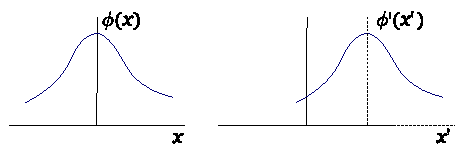
\includegraphics{trasla} %noinstiki
  \caption{Traslaci\'on de funci\'on y coordenadas en una dimensi\'on: $\phi(x)=\phi'(x')$ } %noinstiki
  \label{fig:trasla} %noinstiki
\end{figure} %noinstiki<div id="fig:trasla">Figura trasla:Traslaci\'on de funci\'on y coordenadas $\phi(x)=\phi(x')$ </div>
%noinstiki![trasla](http://gfif.udea.edu.co/figfs/trasla.png)
%noinstiki
Si $a^\mu$ es constante (un an\'alisis m\'as general es hecho en \cite{r})
\begin{equation}
  d^4x'=d^4x
\end{equation}
En este caso, asumiendo que el campo satisface las ecuaciones de
Euler-Lagrange y usando la ec.~\eqref{eq:dmuxmu} y (\ref{eq:eelcallfmu}) tenemos
\begin{align}
  \delta S&=\int_{R}d^4x\,\mathcal{L}(\phi',\partial_\mu\phi',x')-\int_{R}d^4x\,\mathcal{L}(\phi(x),\partial_\mu\phi(x),x)\nonumber\\
  &=\int_{R}d^4x\,\mathcal{L}(\phi+\delta\phi,\partial_\mu\phi+\partial_\mu(\delta\phi),x+\delta a)-\int_{R}d^4x\,\mathcal{L}\nonumber\\
  &\approx\int_{R}d^4x\,
  \left[\mathcal{L}+
    \frac{\partial\mathcal{L}}{\partial\phi}\delta\phi+\frac{\partial\mathcal{L}}{\partial(\partial_\mu\phi)}\partial_\mu(\delta\phi)+
    (\partial_\mu\mathcal{L})\delta a^\mu\right]-\int_{R}d^4x\,\mathcal{L}\nonumber\\
  &=\int_{R}d^4x\,
  \left[
    \frac{\partial\mathcal{L}}{\partial\phi}\delta\phi+\frac{\partial\mathcal{L}}{\partial(\partial_\mu\phi)}\partial_\mu(\delta\phi)+
    (\partial_\mu\mathcal{L})\delta a^\mu\right]\nonumber\\
  &=\int_{R}d^4x\,
  \left\{ 
    \left[\partial_\mu\left(\frac{\partial\mathcal{L}}{\partial(\partial_\mu\phi)}
    \right)\right]\delta\phi+\frac{\partial\mathcal{L}}{\partial(\partial_\mu\phi)}\partial_\mu(\delta\phi)+
    (\partial_\mu\mathcal{L})\delta a^\mu\right\}\nonumber\\
  &=\int_{R}d^4x\left\{ 
    \partial_\mu\left[\frac{\partial\mathcal{L}}{\partial(\partial_\mu\phi)}\delta\phi\right]
  +(\partial_\mu\mathcal{L})\delta a^\mu\right\}\nonumber\\
  &=\int_{R}d^4x\,
    \partial_\mu\left[
      -\frac{\partial\mathcal{L}}{\partial(\partial_\mu\phi)}(\partial_\nu\phi)
      +\delta^\mu_\nu\mathcal{L}
    \right]\delta a^\nu\nonumber\\
    \label{eq:2}
  &=\int_{R}d^4x\,
  \left(
    \partial_\mu T^\mu_\nu
  \right)\delta a^\nu=0.
\end{align}
Y por consiguiente
\begin{equation}
  \label{eq:131}
  \partial_\mu T^\mu_\nu=0,
\end{equation}
donde
\begin{equation}
  \label{eq:tmunu}
    T^\mu_\nu=\frac{\partial\mathcal{L}}{\partial(\partial_\mu\phi)}(\partial_\nu\phi)
      -\delta^\mu_\nu\mathcal{L}
\end{equation}
El tensor $T^\mu_\nu$ proviene de asumir la homogeneidad del espacio y el tiempo y es llamado el tensor de momentum--energ\'\i a. 
La densidad Hamiltonina se obtiene de $T^0_0$
\begin{align}
  \label{eq:3}
\mathcal{H}&=T^0_0=\frac{\partial\mathcal{L}}{\partial\dot{\phi}}\dot{\phi}
      -\mathcal{L}\\
      &=\pi(x)\frac{\partial\phi(x)}{\partial t}-\mathcal{L}.
\end{align}
Comparando con la expresi\'on correspondiente en la formulaci\'on
Lagrangiana de la Mec\'anica Cl\'asica, tenemos que si $\phi(x)$ es la
variable can\'onica, la variable can\'onica conjugada es $\pi(x)$
\begin{equation}
  \label{eq:4}
  \pi(x)=\frac{\partial\mathcal{L}}{\partial(\partial\phi(x)/\partial t)}.
\end{equation}
El teorema de Noether en este caso establece que la invarianza de la Acci\'on bajo traslaciones temporales da lugar a la ecuaci\'on de continuidad (\ref{eq:131}) para $\nu=0$
\begin{align}
\label{eq:122}
  \partial_\mu T^\mu_0=0
\end{align}
cuya carga conservada corresponde a la energ\'\i a
\begin{align}
  H=\int_V d^3x\, T^0_0=\int_V d^3x\,\mathcal{H}.
\end{align}
De igual forma la invarianza bajo traslaciones espaciales de lugar a ecuaciones de continuidad para cada componente $\nu=i$
 ($i=1,2,3$)
 \begin{align}
   \label{eq:235}
   \partial_\mu T^\mu_i=0,
 \end{align}
cuyas densidad de cargas conservadas, $T^0_i$, que en forma vectorial escribiremos como $\mathbf{T}^0$, dan lugar a la conservaci\'on del momentum
\begin{align}
  \mathbf{P}=\int_V d^3x\,\mathbf{T}^0\,.
\end{align}
Generalizando a un campo complejo
\begin{equation}
  \label{eq:138}
     T^\mu_\nu=\frac{\partial\mathcal{L}}{\partial(\partial_\mu\phi)}(\partial_\nu\phi)+(\partial_\nu\phi^*)\frac{\partial\mathcal{L}}{\partial(\partial_\mu\phi^*)}
      -\delta^\mu_\nu\mathcal{L}
\end{equation}

\section{Aplicaci\'on a Mec\'anica Cu\'antica}
\label{sec:aplic-mecan-cuant}

Haciendo $\hbar=1$, el Lagrangiano que da lugar a la ecuaci\'on de Schr\"odinger es
\begin{align}
\label{eq:5}
  \mathcal{L}(\psi,\psi^*,\partial_\mu\psi,\partial_\mu\psi^*)&=\frac{1}{2m}\boldsymbol{\nabla}\psi^*\cdot\boldsymbol{\nabla}\psi-\frac{i}{2}
  \left(
\psi^*\frac{\partial\psi}{\partial t}-\frac{\partial\psi^*}{\partial t}\psi
  \right)+\psi^*V\psi\\
&=\frac{1}{2m}\partial_i\psi^*\partial_i\psi-\frac{i}{2}
  \left(\psi^*\partial_0\psi-\partial_0\psi^*\psi\right)+\psi^*V\psi.\nonumber
\end{align}
Aplicando las ecuaciones de Euler-Lagrange (\ref{eq:132}) para
la funci\'on de onda $\psi^*$ obtenemos la ecuaci\'on de Scr\"odinger con $\hbar=1$:
\begin{equation}
  \label{eq:137}
    0=\partial_\mu\left[\frac{\partial\mathcal{L}}{\partial(\partial_\mu\psi^*)}\right]-\frac{\partial\mathcal{L}}{\partial\psi^*}=
  \partial_0\left[\frac{\partial\mathcal{L}}{\partial(\partial_0\psi^*)}\right]+  
\partial_i\left[\frac{\partial\mathcal{L}}{\partial(\partial_i\psi^*)}\right]-\frac{\partial\mathcal{L}}{\partial\psi^*}.
\end{equation}
Como
\begin{align}
  \label{eq:136}
  &\frac{\partial\mathcal{L}}{\partial(\partial_0\psi)}=-\frac{i}{2}\psi^*&&\frac{\partial\mathcal{L}}{\partial(\partial_0\psi^*)}=\frac{i}{2}\psi\nonumber\\
  &\frac{\partial\mathcal{L}}{\partial(\partial_i\psi)}=\frac{1}{2m}\partial_i\psi^*&&\frac{\partial\mathcal{L}}{\partial(\partial_i\psi^*)}=\frac{1}{2m}\partial_i\psi\\
  &\frac{\partial\mathcal{L}}{\partial\psi}=\frac{i}{2}\partial_0\psi^*+\psi^*V&&\frac{\partial\mathcal{L}}{\partial\psi^*}=-\frac{i}{2}\partial_0\psi+V\psi.\nonumber
\end{align}
Entonces, reemplazando la ec.~(\ref{eq:136}) en la ec.~(\ref{eq:137}), tenemos
\begin{align}
 0=\partial_\mu\left[\frac{\partial\mathcal{L}}{\partial(\partial_\mu\psi^*)}\right]-\frac{\partial\mathcal{L}}{\partial\psi^*}
 &=\partial_0\left(\frac{i}{2}\psi\right)+\partial_i\left(\frac{1}{2m}\partial_i\psi\right)
  -\left(-\frac{i}{2}\partial_0\psi+V\psi\right)\nonumber\\
  &=\frac{i}{2}\partial_0\psi+\frac{1}{2m}\partial_i\partial_i\psi+\frac{i}{2}\partial_0\psi-V\psi.
\end{align}

Que puede escribirse como
\begin{equation}
  \label{eq:133}
  i\frac{\partial}{\partial t}\psi=
  \left(
    -\frac{1}{2m}\nabla^2+V
  \right)\psi.
\end{equation}

El Lagrangiano en ec~(\ref{eq:5}), y por consiguiente la Acci\'on, es invariante bajo una transformaci\'on de fase
\begin{equation}
  \label{eq:6}
  \psi\to\psi'=e^{i\theta}\psi.
\end{equation}
Por consiguiente, de acuerdo al Teorema de Noether, debe existir una cantidad conservada. La corriente conservada se obtine de la ec.~(\ref{eq:jmuphi}). Para los campos $\psi$ y $\psi^*$, tenemos
\begin{align}
  \delta\psi=\psi'-\psi=(e^{i\theta}-1)\psi&\approx i\theta\psi\\
  \delta\psi^*&\approx-i\theta\psi.
\end{align}
Usando adem\'as la ec.~(\ref{eq:136}) en la definici\'on de $J^0$ dada por la ec.~(\ref{eq:jmuphi}), tenemos
\begin{align}
  \label{eq:135}
  J^0&=\left[\frac{\partial\mathcal{L}}{\partial(\partial_0\psi)}\right]\delta\psi
  +\delta\psi^*\left[\frac{\partial\mathcal{L}}{\partial(\partial_0\psi^*)}\right]\nonumber\\
  &=-\frac{i}{2}\psi^*(i\theta\psi)+(-i\theta\psi^*)\frac{i}{2}\psi\nonumber\\
  &=\theta\psi^*\psi,
\end{align}
y
\begin{align}
  \label{eq:134}
  J^i&=\left[\frac{\partial\mathcal{L}}{\partial(\partial_i\psi)}\right]\delta\psi
  +\delta\psi^*\left[\frac{\partial\mathcal{L}}{\partial(\partial_i\psi^*)}\right]\nonumber\\
  &=\frac{1}{2m}\partial_i\psi^*(i\theta\psi)+(-i\theta\psi^*)\frac{1}{2m}\partial_i\psi\nonumber\\
  &=\frac{i\theta}{2m}\left(\partial_i\psi^*\psi-\psi^*\partial_i\psi \right).
\end{align}
Entonces, normalizando apropiadamente la corriente escogiendo $\theta=1$, tenemos
\begin{align}
  \label{eq:7}
  J^0&=\psi^*\psi\\
  \mathbf{J}&=\frac{i}{2m}
  \left(
    \psi\boldsymbol{\nabla}\psi^*-\psi^*\boldsymbol{\nabla}\psi
  \right).
\end{align}
De acuerdo a la ec.~(\ref{eq:7}), la cantidad conservada corresponde a la probabilidad de la funci\'on de onda y normalizando apropiadamente la ec.~(\ref{eq:qcons})
\begin{equation}
  \label{eq:57}
Q_\rho=  \int_V \psi^*\psi \,d^3x=1.
\end{equation}

En cuanto a las simetr\'\i as externas, tenemos de la ec.~(\ref{eq:tmunu}) que
da lugar a las ecuaciones de continuidad (\ref{eq:122})(\ref{eq:235})
\begin{align}
  \partial_\mu T^\mu_0&=0,\nonumber\\
\partial_\mu{T}^\mu_i&=0
\end{align}
Las cargas conservadas corresponden entonces a $T^0_0$ y $T^0_i$.
Usando  las ecs.~(\ref{eq:136}) en la ec.~(\ref{eq:138})
\begin{align}
  T^0_i=&\frac{\partial\mathcal{L}}{\partial(\partial_0\psi)}(\partial_i\psi)
  +(\partial_i\psi^*)\frac{\partial\mathcal{L}}{\partial(\partial_0\psi^*)}\nonumber\\
  T^0_i=&-\frac{i}{2}\psi^*(\partial_i\psi)+\frac{i}{2}(\partial_i\psi^*)\psi
\end{align}
Entonces, definiendo
\begin{equation}
   \mathbf{T}^0=\frac{i}{2}
  \left(
    \psi\boldsymbol{\nabla}\psi^*-\psi^*\boldsymbol{\nabla}\psi
  \right)
\end{equation}
Adem\'as
\begin{align}
 \mathbf{T}^0&=\frac{i}{2}
  \left(
    -\boldsymbol{\nabla}(\psi^*\psi)-\psi^*\boldsymbol{\nabla}-\psi^*\boldsymbol{\nabla}\psi
  \right)\nonumber\\
&=-i\psi^*\boldsymbol{\nabla}\psi+\frac{i}{2}\boldsymbol{\nabla}(\psi^*\psi)\,.
\end{align}
Integrando en el volumen
\begin{equation}
  \int_V \mathbf{T}^0\, d^3x=-i\int_V \psi^*\boldsymbol{\nabla}\psi\, d^3x-\frac{i}{2}\boldsymbol{\nabla}\int_V\psi^*\psi\,d^3x
\end{equation}
De acuerdo a la ec.~(\ref{eq:57}), la \'ultima integral es una constante y
\begin{align}
  \label{eq:140}
  \int_V \mathbf{T}^0\, d^3x=-i\int_V \psi^*\boldsymbol{\nabla}\psi d^3x\nonumber\\
\langle\widehat{\mathbf{p}}\rangle=\int_V \psi^*\widehat{\mathbf{p}}\psi d^3x
\end{align}
De modo que $\langle\widehat{\mathbf{p}}\rangle$ son las cargas conservadas asociadas al valor esperado el operador de momentum
\begin{equation}
  \widehat{\mathbf{p}}=-i\boldsymbol{\nabla}\,.
\end{equation}
De otro lado
\begin{align}
  T^0_0&=\frac{\partial\mathcal{L}}{\partial(\partial_0\psi)}{\partial_0\psi}+{\partial_0\psi^*}\frac{\partial\mathcal{L}}{\partial(\partial_0\psi^*)}-\mathcal{L}\nonumber\\
  &=-\frac{i}{2}\psi^*\partial_0\psi+\frac{i}{2}\partial_0\psi^*\psi-\frac{1}{2m}\partial_i\psi^*\partial_i\psi+\frac{i}{2}
  \left(\psi^*\partial_0\psi-\partial_0\psi^*\psi\right)-\psi^*V\psi\nonumber\\
  &=-\frac{1}{2m}\partial_i\psi^*\partial_i\psi-\psi^*V\psi
\end{align}
Como las corrientes solo est\'an determinadas hasta un factor de proporcionalidad, definimos
\begin{align}
  \label{eq:139}
   \mathcal{H}&\equiv-T^0_0=\frac{1}{2m}\boldsymbol{\nabla}\psi^*\cdot\boldsymbol{\nabla}\psi+\psi^*V\psi\nonumber\\
   &=\frac{1}{2m}\boldsymbol{\nabla}\cdot(\psi^*\boldsymbol{\nabla}\psi)-\frac{1}{2m}\psi^*\nabla^2\psi+\psi^*V\psi.
\end{align}
Integrando sobre el volumen y usando la ec.~(\ref{eq:140})
\begin{align}
 \int_V\mathcal{H}\,d^3x&=\frac{1}{2m}\int_V\boldsymbol{\nabla}\cdot(\psi^*\boldsymbol{\nabla}\psi)
+\int_V\psi^*\left(-\frac{1}{2m}\nabla^2+V\right)\psi\,d^3x\nonumber\\
&=\frac{1}{2m}\boldsymbol{\nabla}\cdot\int_V(\psi^*\boldsymbol{\nabla}\psi)
+\int_V\psi^*\left(-\frac{1}{2m}\nabla^2+V\right)\psi\,d^3x\nonumber\\
&=\frac{i}{2m}\boldsymbol{\nabla}\cdot\langle\widehat{\mathbf{p}}\rangle
+\int_V\psi^*\left(-\frac{1}{2m}\nabla^2+V\right)\psi\,d^3x\nonumber\\
&=\int_V\psi^*\left(-\frac{1}{2m}\nabla^2+V\right)\psi\,d^3x\,.
\end{align}

Entonces
\begin{align}
\label{eq:141}
H&\equiv \int_V\mathcal{H}\,d^3x=\int_V\psi^*\left(-\frac{1}{2m}\nabla^2+V\right)\psi\,d^3x\nonumber\\
&=\int_{V} d^3x\,\psi^*\widehat{H}\psi=\langle\widehat{H}\rangle.
\end{align}
Que es un resultado bien conocido de la mec\'anica cu\'antica.

Como
\begin{equation}
  \widehat H=\frac{1}{2m}\hat p^2+\widehat V,
\end{equation}
podemos escribir la ec.~(\ref{eq:133}) como
\begin{equation}
  i\frac{\partial}{\partial t}\psi=\widehat H \psi\,.
\end{equation}
Podemos identificar entonces los operadores de energ\'\i a y momentum.
\begin{equation}
  \label{eq:151}
  \widehat H=i\frac{\partial}{\partial t},\qquad \hat{\mathbf{p}}=-i\,\boldsymbol{\nabla}.
\end{equation}

Retornando a la ec.~(\ref{eq:140}), tenemos que para la soluci\'on de part\'\i cula libre de la ecuaci\'on de Schr\"odinger 
\begin{equation}
  \psi=A\,e^{-i\mathbf{k}\cdot\mathbf{x}},
\end{equation}
la condici\'on de normalizaci\'on en ec.~\eqref{eq:57} implica que $|A|^2=1/L^3$, y
\begin{align}
  \int_V \mathbf{T}^0\, d^3x&=\mathbf{k}.
\end{align}

N\'otese que de la ec.~(\ref{eq:1 41}) se puede obtener la densidad Hamiltoniana, y usando la ec.~(\ref{eq:3}) se puede encontrar la densidad Lagrangiana



\section{Aplicaci\'on a la cuerda unidimensional}
\label{sec:aplicacion-la-cuerda}

%\textbf{Hacer la disuci\'on de los operadores de creaci\'on y destrucci\'on por lo menos al nivel del libro de Kane}
Para el Lagrangiano en la ec.~(\ref{eq:call2}), la ecuaci\'on de continuidad para la energ\'\i a es
\begin{align}
  \label{eq:239}
  \partial_\mu T^\mu_0&=0\nonumber\\
  \partial_0 T^0_0+\partial_3 T^3_0&=0\nonumber\\
  \frac{\partial\mathcal{H}}{\partial t}+\frac{\partial\mathcal{P}_z}{\partial z}&=0
\end{align}
donde $\mathcal{H}=T^0_0$ es la densidad de energ\'\i a y $\mathcal{P}_z=T^0_3$ es el flujo de energ\'\i a en la direcci\'on $z$ a lo largo de la cuerda. Mientras que la ecuaci\'on de continuidad para la conservaci\'on del momentum es
\begin{align}
   \frac{\partial T^0_3}{\partial t}+\frac{\partial T^3_3}{\partial z}&=0\,.
\end{align}

Entonces el
Hamiltoniano para la cuerda unidimensional se puede obtener de la ec.~(\ref{eq:3})
\begin{align}
  \label{eq:8}
  \mathcal{H}(\partial\phi/\partial t,\partial\phi/\partial z)&=\frac{\partial\mathcal{L}}{\partial(\partial\phi/\partial t)}\frac{\partial\phi}{\partial t}-\mathcal{L}\nonumber\\
  &=\frac{1}{v^2}\left(\frac{\partial\phi}{\partial t}\right)^2-\frac{1}{2}
\left[
  \frac{1}{v^2}\left(\frac{\partial\phi}{\partial t}\right)^2-\left(\frac{\partial\phi}{\partial z}\right)^2
\right]\nonumber\\
  &=\frac{1}{2}
\left[
  \frac{1}{v^2}\left(\frac{\partial\phi}{\partial t}\right)^2+\left(\frac{\partial\phi}{\partial z}\right)^2
\right],
\end{align}
y
\begin{equation}
  \label{eq:142}
  H=\int_{0}^{L}\mathcal{H}\,dz\,.
\end{equation}
De acuerdo al Teorema de Noether,
\begin{equation}
  \frac{\partial H}{\partial t}=0\,,
\end{equation}
que establece la conservaci\'on de la energ\'\i a. Adem\'as
\begin{equation}
  P_z=-\int_{0}^{L}T^0_3\,dz\,.
\end{equation}


La componente $z$ del vector de flujo de energ\'\i a (vector de Poynting)
del campo $\phi$ esta dado por $T^3_0$. De la ecuaci\'on para
$T^{\mu\nu}$~(\ref{eq:tmunu})
\begin{align}
  \mathcal{P}_z&=\frac{\partial\mathcal{L}}{\partial(\partial\phi/\partial z)}(\partial\phi/\partial t)\nonumber\\
&=-\frac{\partial\phi}{\partial z}\frac{\partial\phi}{\partial t}\,.
\end{align}
De otro lado
\begin{align}
  T^0_3&=\frac{\partial\mathcal{L}}{\partial(\partial\phi/\partial t)}(\partial\phi/\partial z)\nonumber\\
&=\frac{1}{v^2}\frac{\partial\phi}{\partial t}\frac{\partial\phi}{\partial z}\,.
\end{align}
La cantidad conservada corresponde en este caso al momentum en la direcci\'on $z$
\begin{align}
  P_z=-\int_V d^3x\,T^0_3\,.
\end{align}

Para encontrar la forma explicita del Hamiltoniano y de $P_z$,
proponemos como soluci\'on general a la ecuaci\'on de onda (\ref{eq:econda1}) 
%QUE PASA CON a_n=0
\begin{equation}
  \label{eq:9}
  \phi(z,t)=\sum_{n=-\infty}^\infty\left(\frac{v^2}{2\omega_n L}\right)^{1/2}
  \left[a_n\,e^{i(k_n z-\omega_n t)}+a_n^*\,e^{-i(k_n z-\omega_n t)}\right],
\end{equation}
Para que se satisfagan las condiciones peri\'odicas $\phi(0,t)=\phi(L,t)$, donde $L$ es la longitud de la cuerda
\begin{align}
  \sum_{n=-\infty}^\infty 
  \left(\frac{v^2}{2\omega_n L}\right)^{1/2}
  \left[a_n\,e^{-i\omega_n t}+a_n^*\,e^{i\omega_n t}\right]=
  \left(\frac{v^2}{2\omega_n L}\right)^{1/2}
  \left[a_n\,e^{i(k_n L-\omega_n t)}+a_n^*\,e^{-i(k_n L-\omega_n t)}\right],
\end{align}
Igualando cada coeficiente $a_n$ (o $a_n^*$)
\begin{align}
  e^{-i\omega_nt}&=e^{i(k_nL-\omega_nt)}\nonumber\\
  e^{ik_nL}&=1
\end{align}
y
\begin{equation}
   k_n=\frac{2\pi n}{L},\qquad n=0,\pm1,\pm2,\ldots\,.
\end{equation}
De la ecuaci\'on de onda, 
\begin{align}
      &\frac{1}{v^2}\frac{\partial^2\phi}{\partial t^2}-\frac{\partial^2\phi}{\partial z^2}=0\,\nonumber\\
&\sum_{n=-\infty}^\infty\frac{1}{v^2}\frac{\partial^2}{\partial t^2}
\left\{\left(\frac{v^2}{2\omega_n L}\right)^{1/2}
  \left[a_n\,e^{i(k_n z-\omega_n t)}+a_n^*\,e^{-i(k_n z-\omega_n t)}\right]\right\}\nonumber\\ 
&-\sum_{n=-\infty}^\infty\frac{\partial^2}{\partial z^2}
\left\{\left(\frac{v^2}{2\omega_n L}\right)^{1/2}
  \left[a_n\,e^{i(k_n z-\omega_n t)}+a_n^*\,e^{-i(k_n z-\omega_n t)}\right]\right\}=0\,.
\end{align}
Igualando para cada coeficiente $a_n$ y $a_n^*$
\begin{align}
 &\frac{1}{v^2}\frac{\partial^2}{\partial t^2}
\left\{\left(\frac{v^2}{2\omega_n L}\right)^{1/2}
  \left[a_n\,e^{i(k_n z-\omega_n t)}+a_n^*\,e^{-i(k_n z-\omega_n t)}\right]\right\}\nonumber\\ 
&-\frac{\partial^2}{\partial z^2}
\left\{\left(\frac{v^2}{2\omega_n L}\right)^{1/2}
  \left[a_n\,e^{i(k_n z-\omega_n t)}+a_n^*\,e^{-i(k_n z-\omega_n t)}\right]\right\}=0\,,
\end{align}
\begin{align}
  &\frac{-i\omega_n}{v^2}\frac{\partial}{\partial t}\left[
      a_n\,e^{i(k_nz-\omega_n t)}-a_n^*\,e^{-i(k_nz-\omega_n t)}\right]\nonumber\\
  &-ik_n\frac{\partial}{\partial z}\left[
      a_n\,e^{i(k_nz-\omega_n t)}-a_n^*\,e^{-i(k_nz-\omega_n t)}\right]=0\,,
\end{align}

\begin{align}
  &\frac{-\omega_n^2}{v^2}\left[
      a_n\,e^{i(k_nz-\omega_n t)}+a_n^*\,e^{-i(k_nz-\omega_n t)}\right]\nonumber\\
  &+k_n^2\left[
      a_n\,e^{i(k_nz-\omega_n t)}+a_n^*\,e^{-i(k_nz-\omega_n t)}\right]=0\nonumber\\
&\left(-\frac{\omega_n^2}{v^2}+k_n^2\right)  
  \left[
    a_n\,\phi_n(z,t)+a_n^*\,\phi_n^*(z,t)
  \right]=0\,,
\end{align}
%\left(\right)
donde
\begin{equation}
   \phi_n(z,t)=\frac{1}{\sqrt{L}}e^{i(k_nz-\omega_nt)}\,.
\end{equation}
Entonces, se debe satisfacer que
\begin{align}
  \label{eq:10}
  \omega_n^2&=v^2k_n^2\nonumber\\
\omega_n^2&=v^2\frac{4\pi^2 n^2}{L^2}\,.
\end{align}
$k_n$ y $\omega_n$ satisfacen
\begin{equation}
  k_{-n}=-k_n,\qquad \omega_{-n}=\omega_n.
\end{equation}

La ecuaci\'on (\ref{eq:9}) queda
\begin{equation}
   \phi(z,t)=\sum_{n=-\infty}^\infty 
  \left(
    \frac{v^2}{2\omega_n}
  \right)^{1/2}
  \left[
    a_n\,\phi_n(z,t)+a_n^*\,\phi_n^*(z,t)
  \right],
\end{equation}
y las funciones $\phi_n$ satisfacen las siguientes condiciones de normalizaci\'on
\begin{equation}
  \int_0^Ldz\,\phi_n^*(z,t)\phi_m(z,t)=\delta_{nm}.
\end{equation}
Adem\'as
\begin{equation}
  \int_0^Ldz\,\phi_n(z,t)\phi_m(z,t)=\delta_{n,-m}e^{-2i\omega_nt}.
\end{equation}

En tal caso de la ec.~(\ref{eq:142}), tenemos (ver problema \ref{item:pch1.1})
\begin{align}
\label{eq:237}
  H&=\frac{1}{2v^2}\int_0^Ldz\,\frac{\partial\phi}{\partial t}\frac{\partial\phi}{\partial t}+
  \frac{1}{2}\int_0^Ldz\,\frac{\partial\phi}{\partial z}\frac{\partial\phi}{\partial z}\nonumber\\
&=\sum_{n=-\infty}^\infty\omega_n\,a_n^*a_n
\end{align}
En unidades naturales donde $\hbar=1$, $E=\hbar\omega=\omega$, y la frecuencia $\omega$ tiene unidades de energ\'\i a. Adem\'as
\begin{equation}
  \label{eq:236}
    P_z=-\int_0^L T^0_3\,dz=\sum_{n=-\infty}^\infty k_n\,a_n^*a_n
\end{equation}
De nuevo el n\'umero de onda representa el vector de flujo de energ\'\i a. 

En una teor\'\i a cu\'antica de campos, el campo $\phi$ pasa a ser un operador
$\hat{\phi}$. Esto puede hacerse de dos maneras. Por el m\'etodo de
cuantizaci\'on can\'onica, usando la variable can\'onica conjuga $\pi(z,t)$
definida en la ec.~(\ref{eq:4}), que para el caso de la cuerda
unidimensional corresponde a
\begin{equation}
  \pi(z,t)=\frac{1}{v^2}\frac{\partial\phi}{\partial t}.
\end{equation}
Entonces los correspondientes operadores para $\phi$ y $\pi$ deben
satisfacer ($\hbar=1$)
\begin{align}
  [\hat{\phi}(z,t),\hat{\pi}(z',t)]&=i\delta(z'-z)\nonumber\\
  \label{eq:11}
  [\hat{\phi}(z,t),\hat{\phi}(z',t)]&=0\\
  [\hat{\pi}(z,t),\hat{\pi}(z',t)]&=0\nonumber
\end{align}
En este caso $\hat{\phi}$, puede expandirse en t\'erminos de los operadores
$\hat a$ y $\hat{a}^\dagger$
\begin{align}
  \label{eq:12}
  \hat{\phi}(z,t)&=\sum_{n=-\infty}^\infty
  \left(
    \frac{v^2}{2\omega_nL}
  \right)^{1/2}
  \left[
    \hat{a}_n\,e^{i(k_nz-\omega_n t)}+\hat{a}^\dagger_n\,e^{i(k_nz-\omega_n t)}
  \right]\nonumber\\
&=\sum_{n=-\infty}^\infty\hat{\phi}_n
\end{align}
y $\hat{\phi}$ y $\hat{\pi}$ satisfacen las relaciones de conmutaci\'on
(\ref{eq:11}) si
\begin{align}
  [\hat{a}_n,\hat{a}^\dagger_n]&=1\nonumber\\
  [\hat a_n,\hat a_n]&=0\nonumber\\
  [\hat{a}^\dagger_n,\hat{a}^\dagger_n]&=0.
\end{align}
El Hamiltoniano es ahora un operador dado por
\begin{equation}
  \widehat{H}=\sum_{n=-\infty}^\infty w_n\widehat{N}_n,
\end{equation}
Con el operador de n\'umero $\widehat{N}_n$, dado por
\begin{equation}
  \widehat{N}_n=\hat{a}^\dagger_na_n.
\end{equation}
Ya que $\widehat{N}_n$ es Herm\'\i tico, \emph{cada} $\widehat{N}_n$ este tiene un conjunto completo de autoestados ortonormales \cite{ultimo}
\begin{align}
  &\widehat{N}_n|m\rangle=m|m\rangle\nonumber\\
  &\langle m'|m\rangle=\delta_{m' m}\nonumber\\
  &\mathbf{1}=\sum_m|m\rangle\langle m|.
\end{align}
Utilizando las relaciones de conmutaci\'on de $\widehat{N}_n$ con $a_n$ y $\hat{a}^\dagger_n$ se puede demostrar que 
\begin{align}
  \hat{a}^\dagger_n|m\rangle&=\sqrt{m+1}\,|m+1\rangle\nonumber\\
  \hat{a}_n|m\rangle&=\sqrt{m}\,|m-1\rangle.
\end{align}
y por consiguiente
\begin{equation}
  \widehat{N}_n|m\rangle=m|m\rangle
\end{equation}
Esto significa que todos los estados se pueden generar desde un estado base $|0\rangle$
\begin{equation}
  |m\rangle=\frac{\left(\hat{a}^\dagger_n\right)^m}{\sqrt{m}!}|0\rangle.
\end{equation}
A los estados $|m\rangle$ se les llama estados de fonones. $m$ corresponde al n\'umero de fonones de energ\'\i a $\omega_n$. $\hat{a}^\dagger_n$ crea un fon\'on de energ\'\i a $\omega_n$, y $a_n$ destruye un fon\'on de frecuencia $\omega_n$. Al estado $|0\rangle$ se le llama el vac\'\i o. 

Para dos operadores de n\'umero de frecuencias diferentes $\omega_{n_1}$ y $\omega_{n_2}$ tenemos
\begin{align}
  \widehat{N}_{n_1}|m_{n_1}\rangle&=m_{n_1}|m_{n_1}\rangle& \widehat{N}_{n_2}|m_{n_2}\rangle&=m_{n_2}|m_{n_1}\rangle\nonumber\\
  \widehat{N}_{n_1}|m_{n_2}\rangle&=0& \widehat{N}_{n_2}|m_{n_1}\rangle&=0.
\end{align}
De este modo
\begin{equation}
  \label{eq:143}
  \widehat{H}|m_{n_1}\rangle=\sum_{n=-\infty}^\infty\omega_{n}\widehat{N}_{n}|m_{n_1}\rangle=\omega_{n_1}m_{n_1}|m_{n_1}\rangle.
\end{equation}


El autoestado del Hamiltoniano para $I$ conjuntos de fonones de diferentes frecuencias puede escribirse como
\begin{equation}
  |m_{n_1},m_{n_2},\ldots,m_{n_I}\rangle.
\end{equation}
A tales estados, con un n\'umero definido de fonones de varias frecuencias, se les llama estados de \emph{Fock}. 

Los autovalores del Hamiltoniano para un estado de Fock son
\begin{equation}
  \widehat{H} |m_{n_1},m_{n_2},\ldots,m_{n_I}\rangle=\sum_{i=1}^I\omega_{n_i}m_{n_i} |m_{n_1},m_{n_2},\ldots,m_{n_i}\rangle,
\end{equation}
de modo que la energ\'\i a de un estado de Fock es
\begin{equation}
  E=\langle m_{n_1},m_{n_2},\ldots,m_{n_I}|\widehat{H} |m_{n_1},m_{n_2},\ldots,m_{n_I}\rangle=\sum_{i=1}^I\omega_{n_i}m_{n_i}.
\end{equation}

Los fonones est\'an asociados a frecuencias, o modos normales de la cuerda, de modo que est\'an relacionados al movimiento de la cuerda como un todo, mientras que las part\'\i culas de la cuerda est\'an localizadas en el espacio de posiciones. En general pueden existir part\'\i culas asociadas a campos abstractos que no tienen conexi\'on con ning\'un sistema mec\'anico. 

Finalmente, si el n\'umero de cuantos de una determinada frecuencia $\omega_{n_1}$ se puede conocer sin ninguna incertidumbre entonces el campo $\phi_{n_1}(z,t)=\langle n_1|\hat{\phi}_{n_1}(z,t)|n_1\rangle$ es completamente incierto. Entre mayor sea la incertidumbre en el n\'umero de fonones de una determinada frecuencia con mayor precisi\'on se podr\'a determinar el campo cl\'asico asociado a esa frecuencia \cite{ultimo}.




Retornando a la ec. \eqref{eq:143} podemos ver que $\hat{\phi}_{n_1}$ puede interpretarse como una part\'\i cula que
transporta una energ\'\i a ($\hbar=1$)
\begin{equation}
  \langle m_{n_1}|\hat{H}|m_{n_1}\rangle=\omega_{n_1}m_{n_1}
\end{equation}
Para una interpretaci\'on completa de part\'\i cula se debe mostrar que el
campo cuantizado tambi\'en transporta momentum. De hecho
\begin{equation}
  \langle m_{n_1}|\hat{P}_z|m_{n_1}\rangle=k_{n_1}m_{n_1}
\end{equation}
La interpretaci\'on del n\'umero de onda de un campo cu\'antico como momentum es m\'as simple en el contexto de la relatividad especial.  La ec.~\eqref{eq:10},
puede interpretarse como la ecuaci\'on energ\'\i a momentum de la
relatividad especial ($c=1$)
\begin{equation}
  \label{eq:13}
  E^2=\mathbf{p}^2+m^2,
\end{equation}
si $m=0$ y $v=c$, es decir, para ondas propagandose
relativ\'\i sticamente
\begin{equation}
  \omega_{n_1}^2=k_{n_1}^2
\end{equation}
El momentum de la part\'\i cula coincide con el correspondiente n\'umero de onda

Entonces, la interpretaci\'on del campo $\hat{\phi}$ como part\'\i cula, es m\'as
directa en un contexto donde se combine la relatividad especial con la
cuantizaci\'on del campo mismo. Obviando estos detalles, en adelante
llamaremos part\'\i cula al campo cl\'asico.

Si modificamos el Lagrangiano en ec.~\eqref{eq:call2}, para incluir un
t\'ermino adicional ($v=c=1$)
\begin{equation}
  \label{eq:14}
  \mathcal{L}(\partial\phi/\partial t,\partial\phi/\partial z)=\frac{1}{2}
\left[
  \left(\frac{\partial\phi}{\partial t}\right)^2-\left(\frac{\partial\phi}{\partial z}\right)^2-m^2\phi^2
\right].
\end{equation}
entonces, la ec.~\eqref{eq:12} es soluci\'on a la ecuaci\'on resultante de
aplicar las ecuaciones de Euler-Lagrange:
\begin{align}
\label{eq:150}
      \frac{\partial^2\phi}{\partial t^2}-\frac{\partial^2\phi}{\partial z^2}+m^2\phi=&0\nonumber\\
      \left(\frac{\partial^2}{\partial t^2}-\frac{\partial^2}{\partial z^2}+m^2
      \right)\phi=&0,
\end{align}
si
\begin{equation}
  \omega^2=k^2+m^2.
\end{equation}
De este modo $m$ puede interpretarse como la masa de la part\'\i cula. 

Generalizando a 3 dimensiones tenemos el Lagrangiano de Klein-Gordon
\begin{equation}
  \label{eq:15}
  \mathcal{L}=\frac{1}{2}
  \left(
\frac{\partial\phi}{\partial t}
  \right)^2-\tfrac{1}{2}\boldsymbol{\nabla}\phi\cdot\boldsymbol{\nabla}\phi-\tfrac{1}{2}m^2\phi^2,
\end{equation}
que dan lugar a la ecuaci\'on de Klein-Gordon

\begin{equation}
\label{eq:152}
  \left(
\frac{\partial^2}{\partial t^2}-\nabla^2+m^2
  \right)\phi=0.
\end{equation}

\section{Problemas}
\label{sec:problemas-2}
\renewcommand{\labelenumi}{\thechapter.\theenumi} %noinstiki
\begin{enumerate}
\item Obtenga el Hamiltoniano a partir de Lagrangiano en\eqref{eq:238} y encuentre la expresi\'on para la densidad Lagrangiana en t\'erminos de $\phi$.
\label{item:pch1.0} %noinstiki
\item Demuestre las ecuaciones (\ref{eq:237})(\ref{eq:236}).
\label{item:pch1.1} %noinstiki

\item \textquestiondown Que cambios se requieren al Lagrangiano de la ecuaci\'on de Dirac para que la Acci\'on sea invariante bajo transformaciones Gauge Locales?. Ver secci\'on \ref{sec:aplic-la-mecan}.



\label{item:pch1.3} %noinstiki

\item A partir del Lagrangiano de la Mec\'anica Cu\'antica invariante bajo transformaciones de fase local encuentre la ecuaci\'on de Schr\"odinger en presencia del campo electromagn\'etico. Ver secci\'on \ref{sec:aplic-la-mecan}.
 



\item Calcule $T^i_0$ para el Lagrangiano de Schr\"odinger
  \begin{align}
    T^i_0=&\frac{\partial\mathcal{L}}{\partial(\partial_i \psi)}\partial_0\psi+\partial_0\psi^*\frac{\partial\mathcal{L}}{\partial(\partial_i \psi^*)}\nonumber\\
    =&\frac{1}{2m}\left(\partial_i\psi^*\partial_0\psi+\partial_0\psi^*\partial_i\psi \right)
  \end{align}
De modo que $T^0_i\neq T^i_0$.

\end{enumerate}


\renewcommand{\labelenumi}{\theenumi} %noinstiki
% \left(\right)
%%% Local Variables: 
%%% mode: latex
%%% TeX-master: "fullnotes"
%%% End: 
